\documentclass{article}

%%%%%%%%%%%%%%%%%%%%%%%%%
% Packages & Macros
%%%%%%%%%%%%%%%%%%%%%%%%%
\usepackage{colortbl}
\usepackage{datetime}
	\newdateformat{monthyeardate}{\monthname[\THEMONTH] \THEYEAR}
\usepackage{graphicx}
\usepackage{hyperref}
\hypersetup{colorlinks,urlcolor=blue}

%%%%%%%%%%%%%%%%%%%%%%%%%
% Tool-Specific Macros
%%%%%%%%%%%%%%%%%%%%%%%%%
\usepackage{xspace}

\newcommand{\args}[1] {\textit{#1}}
\newcommand{\cmd}[1] {\texttt{#1}}     % Use for command window commands, e.g., \cmd{svn up}
\newcommand{\block}[1] {\textsf{#1}}   % Use for Simulink block names, e.g., \cmd{Subsystem1}
\newcommand{\signal}[1] {\textsf{#1}}   % Use for Simulink block names, e.g., \cmd{Subsystem1}
\newcommand{\ring}[1] {\textsf{#1}} 	 % Use for files names and paths
\newcommand{\keyword}[1] {\texttt{#1}} % Use for keywords of programming languages, e.g., \keyword{while}
\newcommand{\file}[1] {\texttt{#1}} 	 % Use for files names and paths
\newcommand{\param}[1] {\textsf{#1}}   % Use for block parameter names, e.g., \param{BlockType}

% Matlab Products
\newcommand{\matlab}{\textsc{Matlab}\@\xspace}
\newcommand{\Matlab}{\textsc{Matlab}\@\xspace}
\newcommand{\Simulink}{Simulink\@\xspace}
\newcommand{\simulink}{Simulink\@\xspace}
\newcommand{\SDV}{Simulink Design Verifier\@\xspace}
\newcommand{\mpath}{\Matlab search path\@\xspace}

% Block Names (not BlockType)
\newcommand{\ds}{\block{Data Store}\@\xspace}
\newcommand{\DSM}{\block{Data Store Memory}\@\xspace}
\newcommand{\DSR}{\block{Data Store Read}\@\xspace}
\newcommand{\DSW}{\block{Data Store Write}\@\xspace}
\newcommand{\DSRW}{\block{Data Store Read/Write}\@\xspace}
\newcommand{\DSMRW}{\block{Data Store Memory/Read/Write}\@\xspace}

\newcommand{\goto}{\block{Goto}\@\xspace}
\newcommand{\from}{\block{From}\@\xspace}

\newcommand{\inport}{\block{Inport}\@\xspace}
\newcommand{\outport}{\block{Outport}\@\xspace}
\newcommand{\constant}{\block{Constant}\@\xspace}
\newcommand{\ground}{\block{Ground}\@\xspace}
\newcommand{\subsystem}{\block{Subsystem}\@\xspace}

\newcommand{\logic}{\block{Logical Operator}\@\xspace}
\newcommand{\relational}{\block{Relational Operator}\@\xspace}
\newcommand{\ifblk}{\block{If}\@\xspace}
\newcommand{\switch}{\block{Switch}\@\xspace}
\newcommand{\merge}{\block{Merge}\@\xspace}

\newcommand{\docblock}{\block{DocBlock}\@\xspace}

\newcommand{\simfunc}{\block{Simulink Function}\@\xspace}
\newcommand{\simfunccaller}{\block{Function Caller}\@\xspace}

\newcommand{\toworkspace}{\block{To Workspace}\@\xspace}
\newcommand{\fromworkspace}{\block{From Workspace}\@\xspace}

\newcommand{\tofile}{\block{To File}\@\xspace}
\newcommand{\fromfile}{\block{From File}\@\xspace}

\newcommand{\fromspreadsheet}{\block{From Spreadsheet}\@\xspace}

\newcommand{\modelref}{\block{Model Reference}\@\xspace}
\newcommand{\library}{\block{Library}\@\xspace}
\newcommand{\librarylink}{\block{Library Link}\@\xspace}

% Commonly used parameters
\newcommand{\AND}{\param{AND}\@\xspace}
\newcommand{\OR}{\param{OR}\@\xspace}
\newcommand{\NOT}{\param{NOT}\@\xspace}
\newcommand{\NOR}{\param{NOR}\@\xspace}
\newcommand{\NAND}{\param{NAND}\@\xspace}
\newcommand{\XOR}{\param{XOR}\@\xspace}
\newcommand{\NXOR}{\param{NXOR}\@\xspace}

% Common Abbreviations
% Example
\newcommand{\eg}{\textrm{e.g.,}\@\xspace}

% That Is To Say
\newcommand{\ie}{\textrm{i.e.,}\@\xspace}

% And So On
\newcommand{\etc}{\textrm{etc.}\@\xspace}

% And Others
\newcommand{\etal}{\textrm{et al.}\@\xspace}

% With Respect To
\newcommand{\wrt}{\textrm{w.r.t.}\@\xspace}

% Vice Versa
\newcommand{\vrsa}{\textrm{vice versa}\@\xspace}

% Symbols

\usepackage{amssymb}
\newcommand{\checkbox}{\makebox[0pt][l]{$\square$}\raisebox{.15ex}{\hspace{0.1em}$\checkmark$}}%
\newcommand{\uncheckbox}{$\square$~}%


\newcommand{\ToolName}{Signature\@\xspace}

\newcommand{\menu}[1]{%
	\ifthenelse{\equal{#1}{1}}{Extract Signature}{}%
  	\ifthenelse{\equal{#1}{2}}{Augment for Test Harness}{}%
}

\newcommand{\func}[1]{%
	\ifthenelse{\equal{#1}{1}}{StrongSignature}{}%
	\ifthenelse{\equal{#1}{2}}{WeakSignature}{}%
	\ifthenelse{\equal{#1}{3}}{TestHarness}{}%
  	\ifthenelse{\equal{#1}{4}}{?}{}%
  	\ifthenelse{\equal{#1}{5}}{?}{}%
  	\ifthenelse{\equal{#1}{6}}{?}{}%
}

\newcommand{\toolFolder}{\cmd{Signature}}
\newcommand{\demoName}{\cmd{SignatureDemo}\@\xspace}

\newcommand{\FCA}{0} 	% Enable/disabled FCA-specific content	
\newcommand{\HowSetPath}{\ifthenelse{\equal{\FCA}{1}}{If it is not, go to \cmd{File~>~Set~Path...}, press \cmd{Add with Subfolders}, and select the \cmd{McMaster\_Tools} folder. Restart \matlab after doing so.}{}}

%%%%%%%%%%%%%%%%%%%%%%%%%
% Document
%%%%%%%%%%%%%%%%%%%%%%%%%

\title{\ToolName Tool}
\date{\monthyeardate\today}

\begin{document}

%%%%%%%%%%%%%%%%%%%%%%%%%%%%%%%%%%%%%%%%%%%%%%%%%%%%%%%%%%%%%%%%%%%
% Title Page
%%%%%%%%%%%%%%%%%%%%%%%%%%%%%%%%%%%%%%%%%%%%%%%%%%%%%%%%%%%%%%%%%%%
\maketitle
\vfill

\begin{figure}
	\centering
	
\includegraphics[]{../figs/McSCert_Logo.pdf} \\
	McMaster Centre for Software Certification (McSCert)
\end{figure}

\newpage

%%%%%%%%%%%%%%%%%%%%%%%%%%%%%%%%%%%%%%%%%%%%%%%%%%%%%%%%%%%%%%%%%%%
% Introduction
%%%%%%%%%%%%%%%%%%%%%%%%%%%%%%%%%%%%%%%%%%%%%%%%%%%%%%%%%%%%%%%%%%%
\section{Introduction}

% Briefly, what is the tool?
A Simulink subsystem has \inport{s} (explicit links to the subsystem), and \outport{s} (explicit links from the subsystem), which are the explicit interface of the subsystem. However, there are usually hidden (implicit) data dependencies across Simulink subsystems. Hidden dependencies originate from two Simulink mechanisms: 1) \DSM; and 2) \goto/\from blocks with a \block{Goto Tag Visibility}\footnote{Called \emph{scoped} \goto/\from blocks}. 

The \ToolName tool extracts the \emph{signature} of a Simulink subsystem. A signature represents the interface of a Simulink subsystem, making all data flow into and out of the subsystem explicit. The tool identifies two types of signatures for a subsystem: \emph{strong} signature and \emph{weak} signature. The strong signature identifies the data mechanisms that \emph{are accessed} by the subsystem or any of its children. The weak signature identifies the data mechanisms that a subsystem \emph{can access} but is not necessarily using (i.e., those which are declared higher up in the hierarchy, and are thus available at lower levels). 

The \ToolName tool can be used to either include the signature in the model itself, or export the signature into a text~(\texttt{.txt}), \TeX~(\texttt{.tex}), or Microsoft Word~(\texttt{.doc}) file. The tool can also be used to improve test harnessing with commercial automatic test generation tools.

% Is there more information?
\subsection*{More Information}
For more about the theoretical background of signatures and how they can be used, an interested reader is referred to:

Marc Bender, Karen Laurin, Mark Lawford, Jeff Ong, Steven Postma, Vera Pantelic, \href{http://www.cas.mcmaster.ca/~lawford/papers/MODELSWARD2014.pdf}{``Signature Required - Making Simulink Dataflow and Interfaces Explicit,"} \textit{Proceedings of 2nd International Conference on Model-Driven Engineering and Software Development (MODELSWARD 2014)}, SCITEPRESS, 2014, 119-131. (Nominated for Best Paper Award)

\vspace{1em}
For more information on the tool and how it can be used in a model-based development with Simulink, please refer to the following papers:

\vspace{1em}
Vera Pantelic, Steven Postma, Mark Lawford, Monika Jaskolka, Bennett Mackenzie, Alexandre Korobkine, Marc Bender, Jeff Ong, Gordon Marks, Alan Wassyng, \href{https://link.springer.com/article/10.1007/s10009-017-0450-9}{``Software engineering practices and Simulink: bridging the gap,"} \textit{International Journal on Software Tools for Technology Transfer (STTT)}, 2017, 95--117.

\vspace{1em}
Vera Pantelic, Steven Postma, Mark Lawford, Alexandre Korobkine, Bennett Mackenzie, Jeff Ong, and Marc Bender, \href{http://www.cas.mcmaster.ca/~lawford/papers/MODELSWARD2015.pdf}{``A Toolset for Simulink: Improving Software Engineering Practices in Development with Simulink,"}\textit{Proceedings of 3rd International Conference on Model-Driven Engineering and Software Development (MODELSWARD 2015)}, SCITEPRESS, 2015, 50--61.

\newpage	
%%%%%%%%%%%%%%%%%%%%%%%%%%%%%%%%%%%%%%%%%%%%%%%%%%%%%%%%%%%%%%%%%%%
% How to Use the Tool
%%%%%%%%%%%%%%%%%%%%%%%%%%%%%%%%%%%%%%%%%%%%%%%%%%%%%%%%%%%%%%%%%%%
\section{How to Use the Tool}
This section describes what must be done to setup the tool, as well as how to use the tool.

%---------------------------------------
% What needs to be done before the tool can be used? 
% What needs to be done to a model in order for it to work on said model?
%---------------------------------------
\subsection{Prerequisites and Installation}

\begin{enumerate}
	\item Use \Matlab/\Simulink 2011b or newer.
	\item To install the tool,
	\begin{enumerate}
		\item from a \file{.zip} file --- unzip the contents into your desired location. Ensure the unzipped folder and subfolders are present in your \mpath, or add them if they are not present. Run \href{https://www.mathworks.com/help/simulink/ug/registering-customizations.html}{sl\_refresh\_customizations} to refresh the Context Menu. 
		\item from a \file{.mltbx} file --- simply open \Matlab and double-click on the file. Your \mpath should be automatically configured.
		\item from the files only --- add the folders and subfolders to your \mpath. Run \href{https://www.mathworks.com/help/simulink/ug/registering-customizations.html}{sl\_refresh\_customizations} to refresh the Context Menu.
	\end{enumerate}
	\begin{itemize}
		\item \textit{Note:} If running the command ``\cmd{which StrongSignature}'' indicates that the script is not found, then the tool needs to be added to the \mpath.
		For information on adding files to the \mpath, please see the \href{https://www.mathworks.com/help/matlab/matlab_env/add-remove-or-reorder-folders-on-the-search-path.html}{MathWorks documentation}.
	\end{itemize}
	\item Ensure the Simulink-Utility folder is on your \mpath. This is a dependency for the tool to work correctly.
	\item Ensure your model is open (or loaded, for command line use) and unlocked.
\end{enumerate}

%---------------------------------------
% How/when do you access the tool?
%---------------------------------------
\subsection{Getting Started}
The tool can be used via the Simulink Context Menu, which can be viewed by right-clicking in a model. The following options are available in the \ToolName menu, as shown in Figure~\ref{FIG:contextMenu}:
\begin{itemize}
	\item \emph{\menu{1}} 
	\item \emph{\menu{2}}
\end{itemize}

\begin{figure}
	\centering
	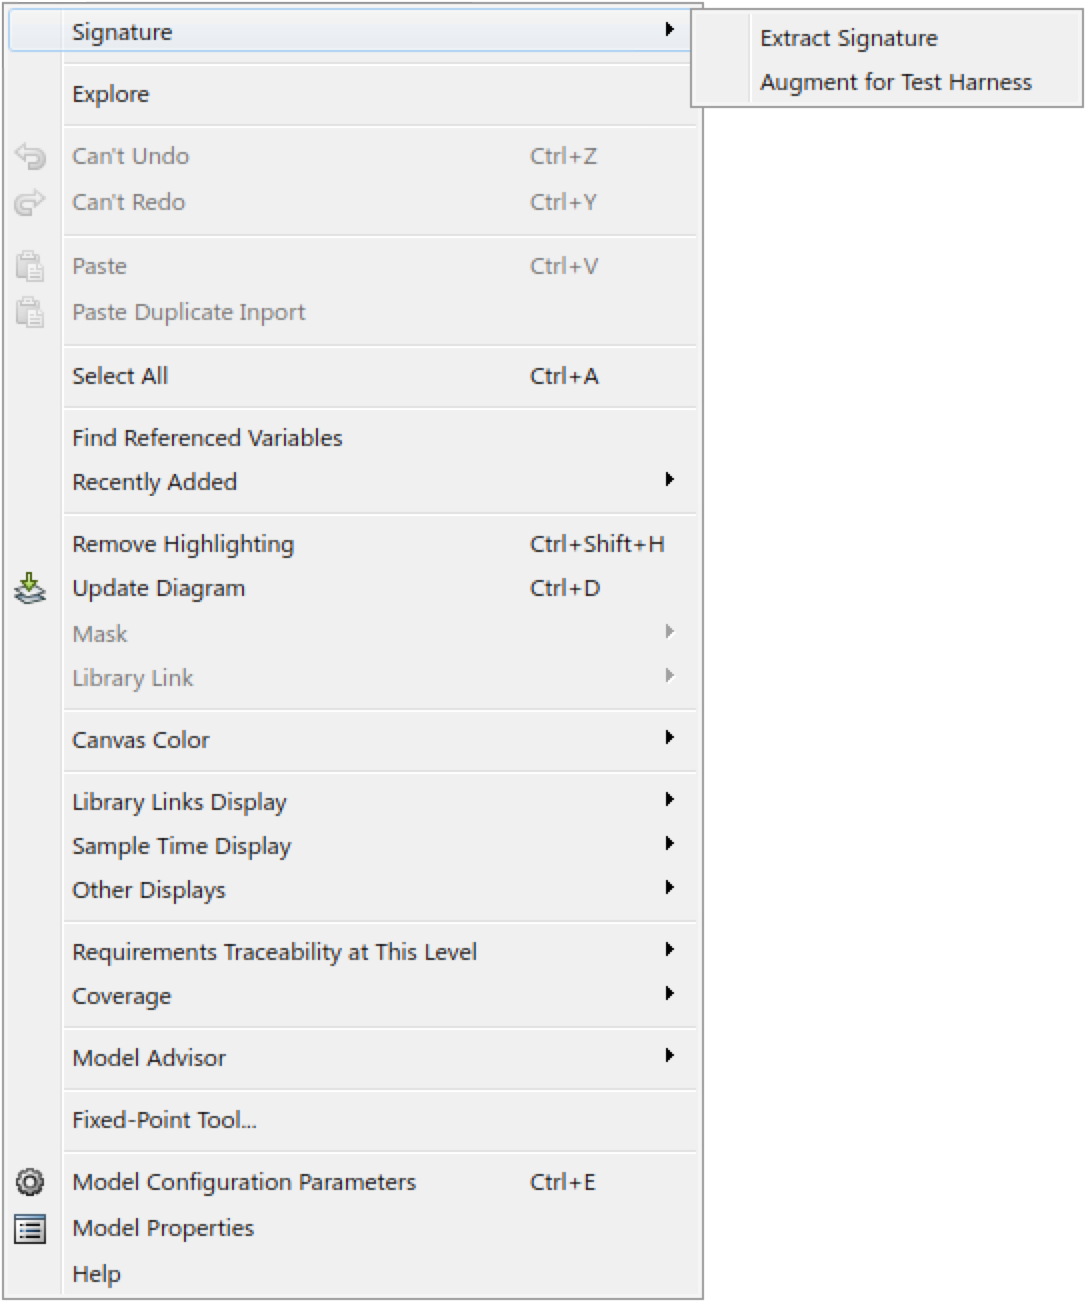
\includegraphics[width=0.7\textwidth]{../figs/ContextMenu}
	\caption{Simulink Context Menu with tool options visible.}
	\label{FIG:contextMenu}
\end{figure}

%---------------------------------------
% What are the main uses of the tool?
%---------------------------------------
\subsection{Functionality}
This section describes the tool functionality when it is used from the Simulink Context Menu (Figure~\ref{FIG:contextMenu}).

\subsubsection*{\menu{1}}
Right-clicking anywhere in the model and then selecting \cmd{\menu{1}} from the Context Menu will display the user interface shown in Figure~\ref{FIG:gui}.

\begin{figure}
	\centering
	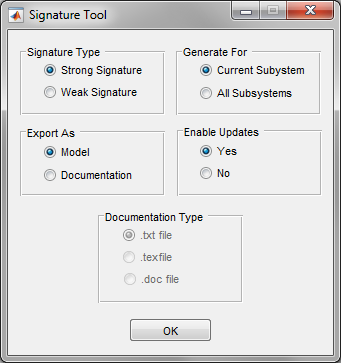
\includegraphics[width=0.5\textwidth]{../figs/GUI}
	\caption{Signature extraction interface.}
	\label{FIG:gui}
\end{figure}

The user has the following options when it comes to generating a signature:

\begin{itemize}
	\item Signature Type --- Choose whether to extract the strong signature or weak signature.
	\item Generator For --- Choose whether to get the signature for the current subsystem (i.e., one level of the hierarchy) or all subsystems.
	\item Export As --- Choose to represent the signature in the model, or as textual documentation.
	\item Enable Updates\footnote{Updates refers to \DSM blocks and scoped \goto/\from blocks that are both written to and read from in a subsystem.}  --- Choose whether updates are to be included in the signature, or included separately as Reads and Writes. \emph{Note:} Do not enable when using with \cmd{\menu{2}}.
	\item Documentation Type --- If exporting as documentation, choose to output as text files, \TeX\,files, or Microsoft Word files.
\end{itemize}	

For signatures generated in the model, a copy of the original model will be created, where the signature will be generated. This new model will have the same filename as the original, with \keyword{\_StrongSig} or \keyword{\_WeakSig} appended. This is done to ensure no changes are made to the original model.

\subsubsection*{\menu{2}}
\paragraph{\emph{Prerequisite:}} The strong signature, without updates, must be generated in the model. Otherwise, this operation will have no effect on the model.
\newline

Right-clicking anywhere in the model and then selecting \cmd{\menu{2}} from the Context Menu, will augment a strong signature for use with test harnessing. This operation is most useful when the subsystem of interest is extracted from the model, with implicit data flow to/from higher levels of the model. Some testing tools, such as Reactis by Reactive Systems, support subsystem extraction in order to test a single subsystem of the model. In this case, implicit data flow information higher in the model may be lost.  Moreover, testing tools commonly do not account for implicit data flow into the subsystem, thereby not generating input data, and ultimately not exercising the model fully. In this situation, depending on the tool and signal type, the value of \from{s}/\DSR{s}  will constantly default to 0 for all tests.

To allow test inputs to be fed into \from{s}/\DSR{s}, or test output data to be recorded from \goto{s}/\DSW{s}, \inport and \outport blocks are added to the strong signature. As a result of these additional \inport{s}/\outport{s}, testing coverage can increase, while testing efforts (e.g., number of test cases) decrease.

\emph{Note:} This operation will have no effect at the root system level, or if the subsystem does not make use of implicit data higher in the hierarchy.

%---------------------------------------
% What are the configuration options for the tool?
%---------------------------------------
\subsection{Configuration Parameters}
The configuration file \cmd{config.txt} is included in \cmd{\toolFolder\textbackslash src}. The following configuration parameters are utilized by the tool, and can be modified by the user in order to tailor tool functionality:

\begin{itemize}
	\item \cmd{gotofrom\_bgcolor} -- The color of the \goto/\from blocks in the signature, and their corresponding \goto/\from blocks connecting the signature to the original model. 
	\item \cmd{heading\_size} -- The font size for the signature section heading annotations (i.e., ``Inputs", ``Outputs", ``Test Harness").
\end{itemize}

Please see the configuration file for more details regarding parameter usage and accepted values. These parameters can be modified with \matlab open, and do not require that \matlab be restarted for the changes to take effect.

%---------------------------------------
% What else does the tool do?
%---------------------------------------
\subsection{Errors and Warnings}
Any errors or warnings during tool use will be visible in the \matlab Command Window. Typically, errors will be shown when the model is locked or function parameters are incorrect.

%%%%%%%%%%%%%%%%%%%%%%%%%%%%%%%%%%%%%%%%%%%%%%%%%%%%%%%%%%%%%%%%%%%
% Example
%%%%%%%%%%%%%%%%%%%%%%%%%%%%%%%%%%%%%%%%%%%%%%%%%%%%%%%%%%%%%%%%%%%
\section{Example}

Use the command \demoName in the Simulink command window to open the example model, shown in Figure~\ref{FIG:demo1}. This example has implicit data flow passing to other levels of the model via \block{Data Store}s, as well as a scoped \goto/\from blocks. In particular, we will focus on \block{Subsystem1}, which is shown in Figure~\ref{FIG:demo1b}. The following steps will demonstrate the various functions of the tool.

\begin{figure}
	\centering
	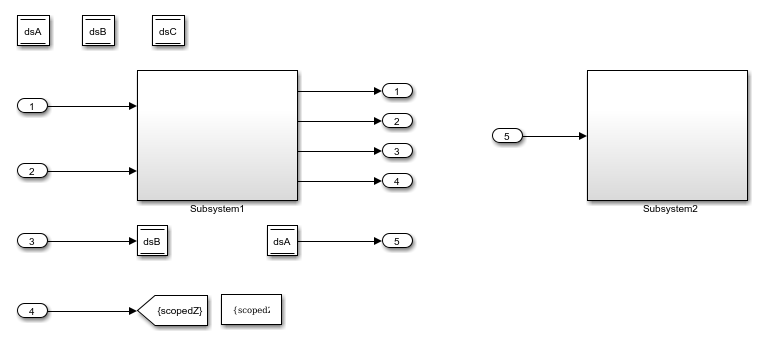
\includegraphics[width=\textwidth]{../figs/Demo1}
	\caption{\ToolName demo: Root level of \demoName.}
	\label{FIG:demo1}
\end{figure}

\begin{figure}
	\centering
	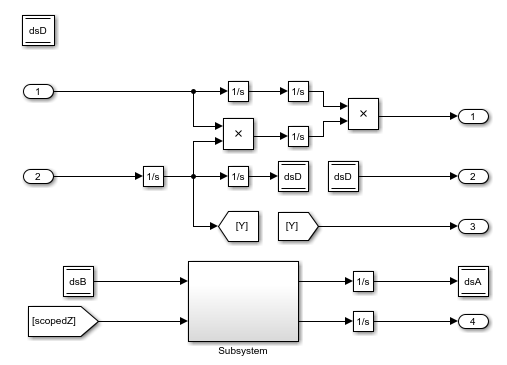
\includegraphics[width=0.65\textwidth]{../figs/Demo1b}
	\caption{\ToolName demo: \block{Subsystem1} from Figure~\ref{FIG:demo1}.}
	\label{FIG:demo1b}
\end{figure}

\begin{enumerate}
	\item \textbf{Generate Strong Signature} Let us extract the strong signature of \block{Subsystem1}. To do this, right-click anywhere in the model and select the \cmd{\menu{1}} option. The \ToolName GUI will pop-up (shown in Figure~\ref{FIG:gui}). Change the \cmd{Export As} option to \cmd{Model}. The resulting model is shown in Figure~\ref{FIG:demo2} and is named \keyword{\demoName{}\_StrongSig.mdl}.
	
	Recall that the strong signature shows all the data that is actually used in the system. Straightforwardly, the \inport{s} and \outport{s} of the subsystem are part of the signature, as these are the typical inputs and outputs of the subsystem. Likewise, the subsystem's use of the \DSR block \block{dsB}, scoped \from block \block{scopedZ}, and \DSW block \block{dsA} are reflected in the signature. Lastly, the \DSM block \block{dsD} is included on the signature, as it is read/written to inside \block{Subsystem}.
	\end{enumerate}

\begin{figure}[ht!]
	\centering
	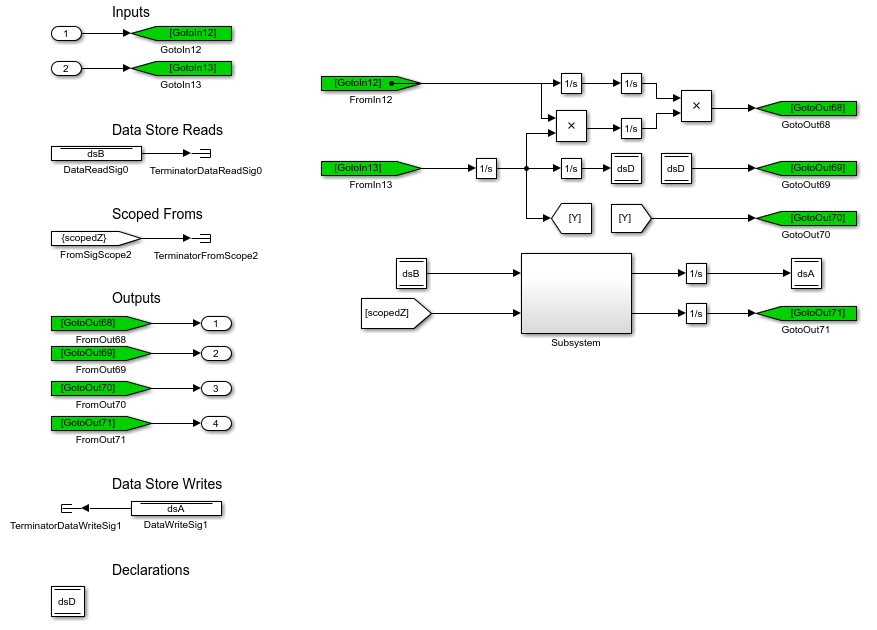
\includegraphics[width=\textwidth]{../figs/Demo2}
	\caption{Strong signature (shown in the model) for Figure~\ref{FIG:demo1b}.}
	\label{FIG:demo2}
\end{figure}

\begin{enumerate}
	\item[2.] \textbf{Generate Weak Signature} Let us now extract the weak signature of \block{Subsystem1}. To do this, right-click anywhere in the original model and select the \cmd{\menu{1}} option. The \ToolName GUI will pop-up (shown in Figure~\ref{FIG:gui}). Change the \cmd{Signature Type} to \cmd{Weak Signature} and change the \cmd{Export As} option to \cmd{Model}. For demonstration purposes, also select \cmd{No} for the \cmd{Enable Updates} option (this will be explained in Step 3). The resulting model is shown in Figure~\ref{FIG:demo3} and is named \keyword{\demoName{}\_WeakSig.mdl}.
	
		In contrast to the strong signature, the weak signature shows all the data that the system \emph{can access}, regardless of if it is actually used. All the information that was in the strong signature is also in the weak signature. For this reason, we again see the \inport{s} and \outport{s} of the subsystem, as well as the \DSR block \block{dsB}, scoped \from block \block{scopedZ}, \DSW block \block{dsA}, and \DSM block \block{dsD} are present, as they are all  read/written to in \block{Subsystem1}.
		
		Due to the presence of \DSM blocks \block{dsA} and \block{dsC} at the root level, this subsystem has the ability to read or write to this memory (although it is currently not doing so). For this reason, \block{dsA} and \block{dsC} are included in the weak signature under the Data Store Read and Data Store Write headings. Moreover, although \block{Subsystem1} is already reading from \DSM \block{dsB}, it has the potential to also write to it. Therefore, \block{dsB} is now also now found under the Data Store Writes heading. 
		
		If at any point in development the use of implicit data items found in the weak signature (and not in the strong signature) is needed, a developer can simply replace the \block{terminator} block connected to the element with a \goto or \from block (depending on the scenario), and easily use the element in their subsystem. The benefit of the weak signature is that it notifies the developer of data that is already available to them.
		
\clearpage

\end{enumerate}

\begin{figure}[ht!]
	\centering
	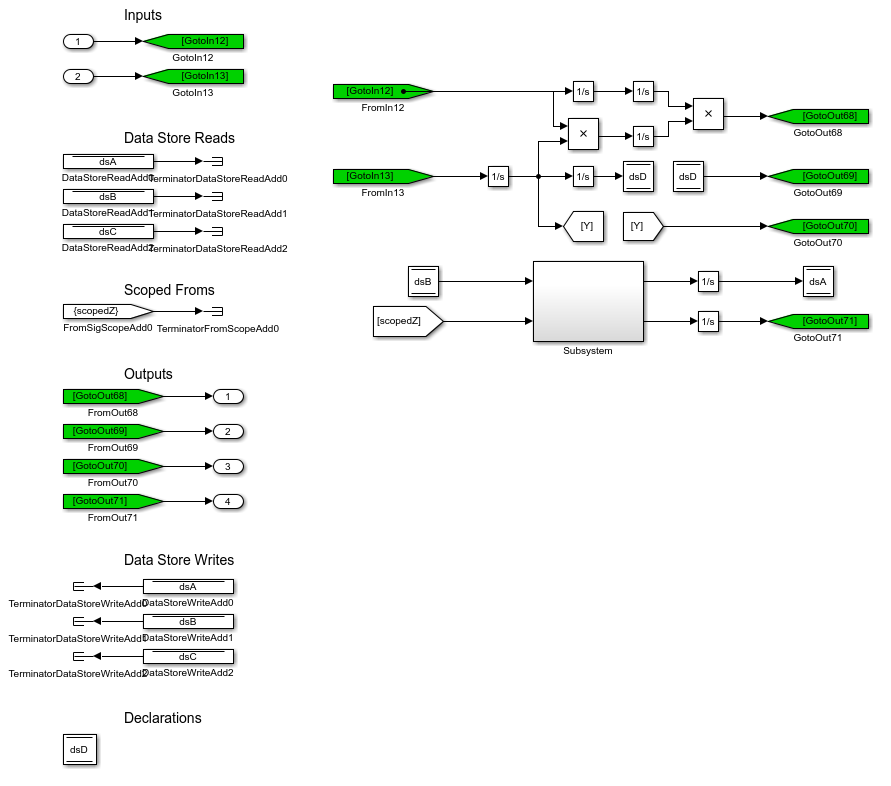
\includegraphics[width=\textwidth]{../figs/Demo3}
	\caption{Weak signature (shown in the model) for Figure~\ref{FIG:demo1b}.}
	\label{FIG:demo3}
\end{figure}

\begin{enumerate}
	\item[3.] \textbf{Generate Signature with Updates} Let us re-generate the weak signature as done in Step 3, but this time with the \cmd{Enable Updates} option set to \cmd{Yes}. The difference in the signature shown in Figure~\ref{FIG:demo4}. In general, for \DSM and scoped \goto/\from blocks that are both read from and written to in the subsystem, will appear together as ``Updates" when enabled. In Figure~\ref{FIG:demo4}, Data Store \block{dsA}, \block{dsB}, and \block{dsC} in the right signature are now grouped together under the Updates heading in the right signature. Updates can be enabled or disabled for both the weak and strong signatures.
\end{enumerate}

\begin{figure}[h!]
	\centering
	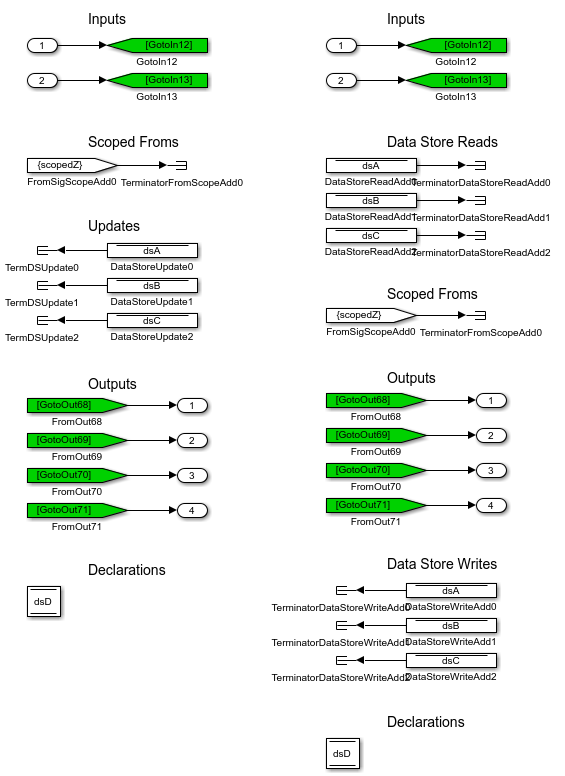
\includegraphics[width=0.8\textwidth]{../figs/Demo4}
	\caption{Difference in signatures between updates enables/disabled.}
	\label{FIG:demo4}
\end{figure}

\begin{enumerate}
	\item[4.] \textbf{Augmenting for Test Harness} To augment a signature for use with a test harness, first the strong signature must be generated in the model with updates disabled. Once this is done, navigate to the system which requires testing. Right-click in the model and select the \cmd{\menu{2}} option. The resulting subsystem is shown in Figure~\ref{FIG:demo5}. The strong signature now contains a new ``Inputs for Harness" section which provides \inport{s} for \block{dsB} and \block{scopeZ} so that testing will generate inputs for the implicit data, thereby exercising the subsystem more thoroughly during testing. Also included is an \outport for \block{dsA}, so that its data can be recorded during testing.
\end{enumerate}

\begin{figure}[ht!]
	\centering
	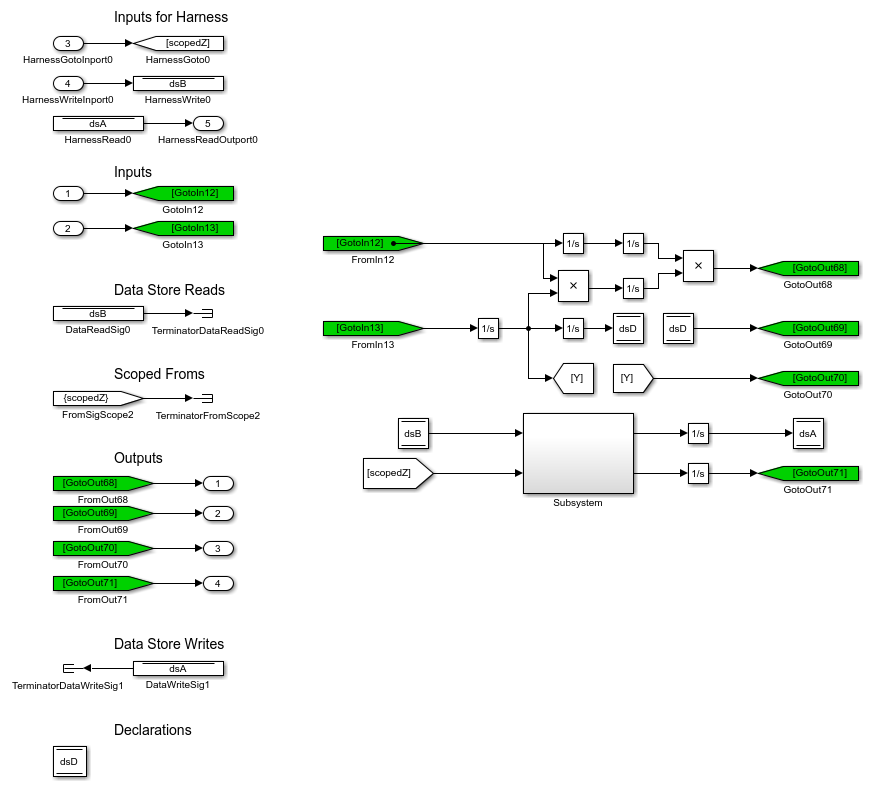
\includegraphics[width=\textwidth]{../figs/Demo5}
	\caption{\block{Subsystem1} of Figure~\ref{FIG:demo1b} augmented for testing.}
	\label{FIG:demo5}
\end{figure}

%%%%%%%%%%%%%%%%%%%%%%%%%%%%%%%%%%%%%%%%%%%%%%%%%%%%%%%%%%%%%%%%%%%
% Matlab Commands
%%%%%%%%%%%%%%%%%%%%%%%%%%%%%%%%%%%%%%%%%%%%%%%%%%%%%%%%%%%%%%%%%%%
\clearpage
\section{Matlab Commands}

The tool can also be used via the \matlab command line, with the following functions.

%---------------------------------------
% Command 1
%---------------------------------------
\begin{center}
	\begin{tabular}{| >{\columncolor[gray]{0.9}}l | p{10.5cm} |} \hline
		Function 		& \cmd{\func{1}} \\ \hline
		Syntax			& \cmd{[metrics, signatures] = \func{1}}(\args{address, exportType, hasUpdates, system, docFormat}) \\ \hline
		Description		& Generate the strong signature for \args{system}. \\ \hline
		Inputs			& \args{address}: Simulink model name. \\[.5em]
						& \args{exportType}: Number indicating whether to export as a model (0) or as documentation (1). \\[.5em] 
						& \args{hasUpdates}: Number indicating whether reads and writes in the same subsystem are kept separate (0), or combined and listed as an update (1). \\[.5em]
						& \args{system}: Name of the system to generate the documentation for. It can be a specific subsystem name, or `All' to document the entire hierarchy. \\[.5em]
						& \args{docFormat}: Number indicating which docmentation type to generate: \texttt{no doc} (0), \texttt{.txt} (1), \texttt{.tex} (2), \texttt{.doc} (3), else no doc. This parameter does not have an impact when \args{exportType} is 0.\\ \hline
		Outputs			& \args{metrics}: Cell array listing the systems and the sizes of their signatures (i.e. number of elements in the signature). \\[.5em]
						& \args{signatures}: Cell array of signature data for the system and its subsystems. Signature data includes: Subsystem, Size, Inports, Outports, ScopedFromTags, ScopedGotoTags, DataStoreReads, DataStoreWrites, Updates, GotoTagVisibilities, and DataStoreMemories.\\ \hline	
	\end{tabular}
\end{center}

%---------------------------------------
% Command 2
%---------------------------------------
\begin{center}
	\begin{tabular}{| >{\columncolor[gray]{0.9}}l | p{10.5cm} |} \hline
		Function 		& \cmd{\func{2}} \\ \hline
		Syntax			& \cmd{[metrics, signatures] = \func{2}}(\args{address, exportType, hasUpdates, system, docFormat}) \\ \hline
		Description		& Generate the weak signature for \args{system}. \\ \hline
		Inputs			& \args{address}: Simulink model name. \\[.5em]
						& \args{exportType}: Number indicating whether to export as a model (0) or as documentation (1). \\[.5em]
						& \args{hasUpdates}: Number indicating whether reads and writes in the same subsystem are kept separate (0), or combined and listed as an update (1). \\[.5em]
						& \args{system}: Name of the system to generate the documentation for. It can be a specific subsystem name, or `All' to document the entire hierarchy. \\[.5em]
						& \args{docFormat}: Number indicating which docmentation type to generate: \texttt{no doc} (0), \texttt{.txt} (1), \texttt{.tex} (2), \texttt{.doc} (3), else no doc. This parameter does not have an impact when \args{exportType} is 0.\\ \hline
		Outputs			& \args{metrics}: Cell array listing subsystems and the sizes of their signatures (i.e., number of elements in the signature). \\[.5em]
						& \args{signatures}: Cell array of signature data for each subsystem. Signature data includes: Subsystem, Size, Inports, Outports, GlobalFroms, GlobalGotos, ScopedFromTags, ScopedGotoTags, DataStoreReads, DataStoreWrites, Updates, GotoTagVisibilities, and DataStoreMemories.\\ \hline	
	\end{tabular}
\end{center}

%---------------------------------------
% Command 3
%---------------------------------------
\begin{center}
	\begin{tabular}{| >{\columncolor[gray]{0.9}}l | p{10.5cm} |} \hline
		Function 		& \cmd{\func{3}} \\ \hline
		Syntax			& \cmd{\func{3}}(\args{system}) \\ \hline
		Description		& Augment \args{system} with a test harness. \\ \hline
		Inputs 			& \args{system}: Simulink system path to generate the harness for. \\ \hline	
		Outputs			& N/A \\ \hline
		%Side Effect	& System is modified with the addition of a test harness. \\ \hline
	\end{tabular}
\end{center}

%%---------------------------------------
%% Command 4
%%---------------------------------------
%\begin{center}
%	\begin{tabular}{| >{\columncolor[gray]{0.9}}l | p{10.5cm} |} \hline
%		Function 		& \\ \hline
%		Syntax			& \\ \hline
%		Description		& \\ \hline
%		Inputs			& \\ \hline	
%		Outputs 		& \\ \hline	
%	\end{tabular}
%\end{center}


%%%%%%%%%%%%%%%%%%%%%%%%%%%%%%%%%%%%%%%%%%%%%%%%%%%%%%%%%%%%%%%%%%%
% Example
%%%%%%%%%%%%%%%%%%%%%%%%%%%%%%%%%%%%%%%%%%%%%%%%%%%%%%%%%%%%%%%%%%%

%\vspace{2em}
%
%\paragraph{Example:} The following commands perform the same operations as described previously for the \demoName example, however via the Matlab command line.
%
%\begin{enumerate}
%	\item \cmd{open\_system(`\demoName')}	
%	\item \cmd{\func{2}(`\demoName', 0, 0, `All', 0)}
%	\item \cmd{\func{1}(`\demoName', 1, 1, `All', 0)} 										
%	\item \cmd{\func{3}(`\demoName')}								
%\end{enumerate}

\end{document}